% XeLaTeX

\documentclass{article}
\usepackage{ctex}
\usepackage{xypic}
\usepackage{amsfonts,amssymb}
\usepackage{multirow}
\usepackage{geometry}
\usepackage{graphicx}
\usepackage{listings}
\usepackage{lipsum}
\usepackage{courier}
\usepackage{fancyvrb}
\usepackage{etoolbox}

\linespread{1.2}
\geometry{left=3cm,right=2.5cm,top=2.5cm,bottom=2.5cm}

\makeatletter
\patchcmd{\FV@SetupFont}
  {\FV@BaseLineStretch}
  {\fontencoding{T1}\FV@BaseLineStretch}
  {}{}
\makeatother

\lstset{basicstyle=\small\fontencoding{T1}\ttfamily,breaklines=true}
\lstset{numbers=left,frame=single,tabsize=4}
%\lstset{extendedchars=false}
\begin{document}

\title{机器学习 AnglesAndDemons 实验报告}
\author {数据科学与计算机学院 \ 计算机科学与技术 2016 级 \\ 王凯祺 \ 16337233}
\maketitle

\section{使用的系统 + 编码语言 + 环境说明}

操作系统:macOS Mojave

代码语言:Python 3、C++

环境说明:第一种为神经网络方法,依赖 Pandas、Numpy、Tensorflow 库;第二种为线性回归方法,依赖 Pandas、Numpy 库。

\section{简单的流程图}

\subsection{数据处理方法}

\subsubsection{观察数据特征}

拿到数据后,第一步是用 Microsoft Excel 打开来看数据的特征。

train.csv 包含 $76901$ 行、 $248$ 列,包含各种各样的数据,有整数类型、浮点数类型、字符串类型,也有缺失值。

label.csv 包含 $76901$ 行,为数据集 train.csv 的标签。标签为 $0$ 或 $1$ 。其中,训练集标签为 $0$ 的占比 $90.86\%$ ,标签为 $1$ 的占比 $9.14\%$ 。

test.csv 包含 $19226$ 行、 $248$ 列,数据类型同 train.csv 。

\subsubsection{数据处理}

第二步是根据数据的特征,进行数据标准化。将字符串映射成整数(相同的字符串映射成相同的整数,不同的字符串映射成不同的整数),然后将数据中的所有整数均视为浮点数。记 max 为列的最大值、 min 为列的最小值,将数据中矩阵的每个元素 $x$ 修改为 $\frac{x - \text{min}}{\text{max} - \text{min}}$ 。这样表格中所有的值都被映射到 $[0, 1]$ 的实数区间。

数据标准化流程图:

\begin{figure}[!h]
\centering
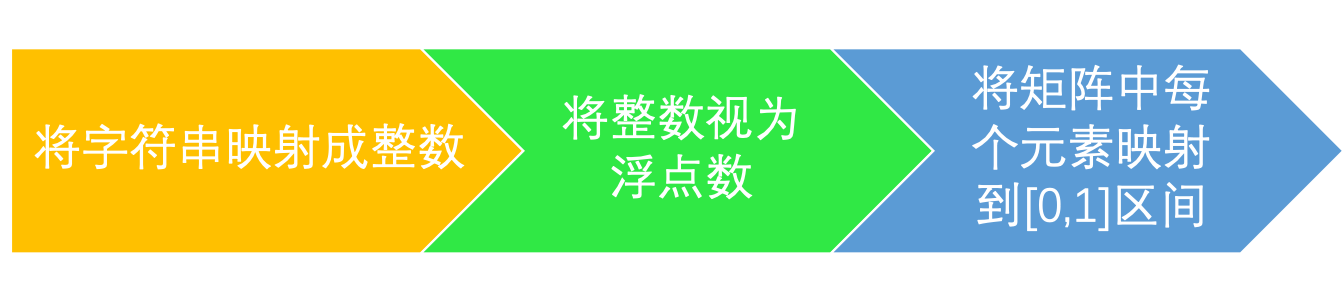
\includegraphics[scale=0.5]{1.png}
\end{figure}

\subsection{选择模型}

在本次作业中,要解决的问题是二分类问题。在我的知识范围内,有两种模型能很好地解决二分类问题:神经网络模型和逻辑回归模型。

\subsubsection{神经网络模型}

在 Tensorflow 的官方文档中,示例代码使用的是神经网络模型来对 $28 \times 28$ 的手写 $'0' - '9'$ 字符进行分类,取得 $93\%$ 左右的准确率。

首先,我们构建一个两层的神经网络结构(输入层 + 输出层)。输入层有训练集列数( $248$ 列 )个节点,输出层有 $2$ 个节点,参数矩阵 $W$ 大小为 $248 \times 2$ ,$b$ 大小为 $2$ 。

接下来,将参数矩阵 $W, b$ 初始化为在 $[-1, 1]$ 内均匀分布矩阵。

定义损失函数为交叉熵,训练使用的方法是梯度下降法,学习率暂定为 $0.01$ 。每训练一次,测试一下准确率。最后输出预测结果。

流程图如下:

\begin{figure}[!h]
\centering

\includegraphics[scale=0.5]{2.png}
\end{figure}

核心代码如下:

\begin{lstlisting}[language=python]
with tf.Session() as sess:
	x = tf.placeholder(tf.dtypes.float32, [None, num_cols]) # 训练集 placeholder
	W = tf.Variable(tf.random_uniform([num_cols, 2], -1.0, 1.0)) # 参数矩阵 W
	b = tf.Variable(tf.random_uniform([2], -1.0, 1.0)) # 参数矩阵 b
	y = tf.nn.softmax(tf.matmul(x, W) + b) # 预测函数
	y_ = tf.placeholder(tf.dtypes.float32, [None, 2]) # 训练集标签
	cross_entropy = tf.reduce_mean(-tf.reduce_sum(y_ * tf.log(y), reduction_indices=[1])) # 交叉熵
	train_step = tf.train.GradientDescentOptimizer(0.01).minimize(cross_entropy)
		# 训练过程
	correct_prediction = tf.equal(tf.argmax(y, 1), tf.argmax(y_, 1))
	accuracy = tf.reduce_mean(tf.cast(correct_prediction, tf.dtypes.float32))
		# 正确率
	test_step = tf.matmul(x, W) + b # 测试集预测
	sess.run(tf.global_variables_initializer()) # 初始化
	validate_data, validate_label = get_validate_value(train_data, train_label, train_num, num_rows) # 验证集
	for t in range(0, 5000):
		data, label = get_train_value(train0, train1)
		sess.run(train_step, {x: data, y_: label}) # 训练
		result = sess.run(accuracy, {x:validate_data, y_: validate_label}) # 计算准确率
		print(t, ' ', result)
	data = get_test_value(test_data)
	result = sess.run(test_step, {x:data}) # 测试集预测
\end{lstlisting}

我测试时每次迭代直接从训练集中抽取 $64$ 个作为本次迭代的训练集。结果发现,预测准确率 $90\%+$ ,但预测结果全部为 $0$ ,这是因为训练集里有太多的 $0$ ,为了得到更高的准确率发生过拟合现象。我想了个办法,将训练集中标签为 $0$ 的随机抽 $32$ 个、标签为 $1$ 的随机抽 $32$ 个作为本次迭代的训练集,不再有过拟合现象。我将二分类的结果(仅含 0、1 的整数)提交,得到 AUC 为 $0.79747$ 。

下面考虑如何输出概率值。由于输出层得到的值有可能是正数,也有可能是负数,我们考虑把输出层得到的数 $+10$ 后跟 $0$ 取最大值,然后将 $\frac{result_1}{result_0 + result_1}$ 作为输出。如此,我把 AUC 提高到了 $0.90510$ 。我们又考虑另一种输出概率的方法,将 $\frac{e^{result_1}}{e^{result_0} + e^{result_1}}$ 作为输出,AUC 提高到 $0.91341$ 。

\subsubsection{线性回归模型}

二层神经网络模型的 AUC 非常有限,再优化也不会比 $0.91$ 多太多,而当前榜单上最高的 AUC 值已经远超过 $0.91$ ,故我选择更换线性回归模型来解决。

我们定义 $248$ 维的列向量 $W$ 以及一个参数 $b$ 。根据书本上的推导,我们需要最大化“对数似然” $$l(w, b) = \sum\limits_{i=1}^{m} \ln p(y_i | x_i; w, b)$$

对 $w$ 求导:
$$\frac{\partial l(w, b)}{\partial w} = \sum\limits_{i=1}^{m} (\frac{e^{W^TX_i + b}}{1 + e^{W^TX_i + b}} - y_i) X_i^{(j)}$$

故 $w$ 的更新:
$$W_{new}^{(j)} = W^{(j)} - \eta \sum\limits_{i=1}^{m} (\frac{e^{W^TX_i + b}}{1 + e^{W^TX_i + b}} - y_i) X_i^{(j)}$$

流程图如下:

\begin{figure}[!h]
\centering
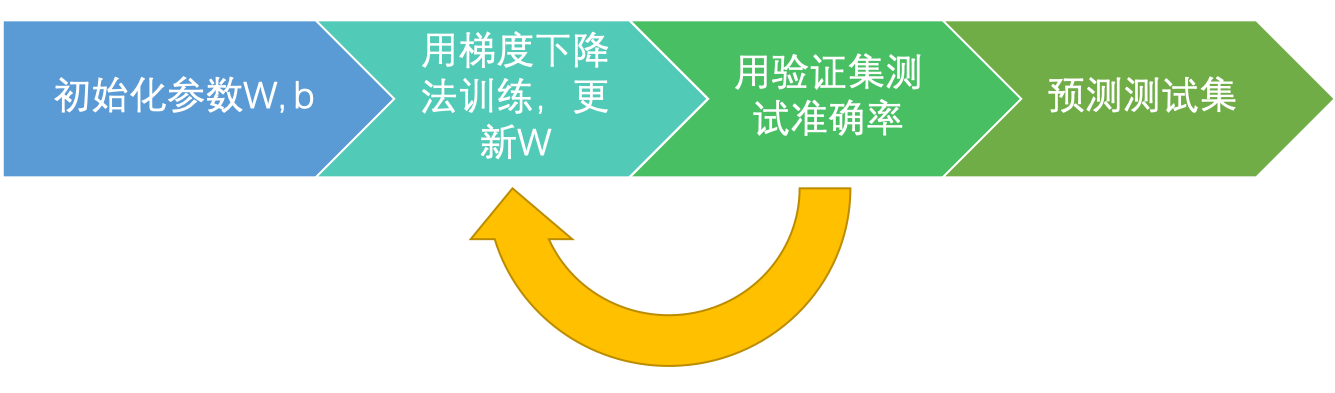
\includegraphics[scale=0.5]{3.png}
\end{figure}

核心代码如下:

\begin{lstlisting}[language=python]
for t in range(0, 1000000):
	data, label = get_train_value(train0, train1) # 取训练集
	d1 = np.zeros([num_cols + 1, 1])
	for i in range(0, BATCH_SIZE):
		x = data[i].reshape([num_cols + 1, 1])
		pp = p1(x, W.reshape([1, num_cols + 1]))
		tt = (pp - label[i]) * x
		d1 = d1 + tt # 计算导数
	W = W - learning_rate * d1 # 更新 W
\end{lstlisting}

\subsubsection{线性回归模型 + Bagging}

只用线性回归模型做出来的结果还不够好,最佳 AUC 仅为 $0.95174$ 。我思考是否能通过集成学习的手段提高 AUC ,第一个想到的就是 Bagging ,因为 Bagging 只需要对现有的结果进行简单的加权计算,而不需要重新训练模型。具体做法是:先训练模型,每迭代一定次数输出预测结果,然后再将这些结果取平均 / 中位数。

流程图如下:

\begin{figure}[!h]
\centering
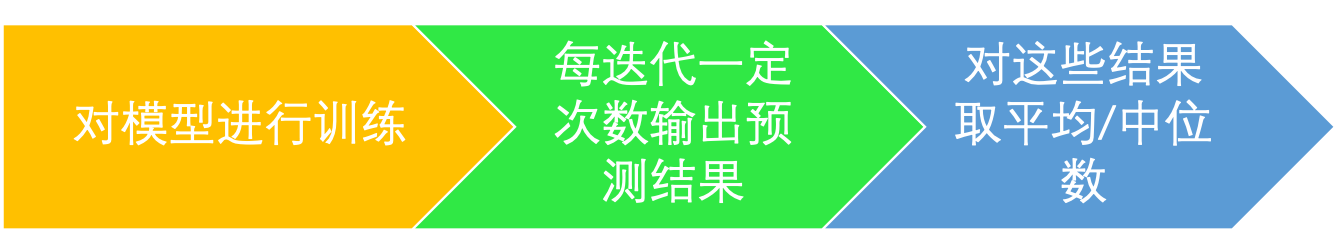
\includegraphics[scale=0.5]{4.png}
\end{figure}

我们每迭代 $3000$ 次就输出一次预测结果。在迭代 $3 \times 10^5$ 次后,我们拿到了 $100$ 份结果。我们对这些结果取平均值后提交, AUC 为 $0.95174$ ;取中位数后提交,AUC 为 $0.95176$ 。Bagging 能综合每个模型的优点,取得这些模型 AUC 中的上确界,但是对 AUC 的提升无明显作用。

\subsubsection{线性回归模型 + AdaBoost}

Bagging 对模型的提升非常有限,我又尝试了 Boosting 。书上介绍了 AdaBoost 算法,我在此进行了尝试。

AdaBoost 算法大致是这样工作的:每次训练一个模型,然后用模型预测一次训练集。若正确则在下一次的训练集中它的比重降低,若错误则在下一次的训练集中它的比重提高。然后将每次训练的结果按照与错误率有关的函数的权值加权求平均值。

流程图如下:

\begin{figure}[!h]
\centering
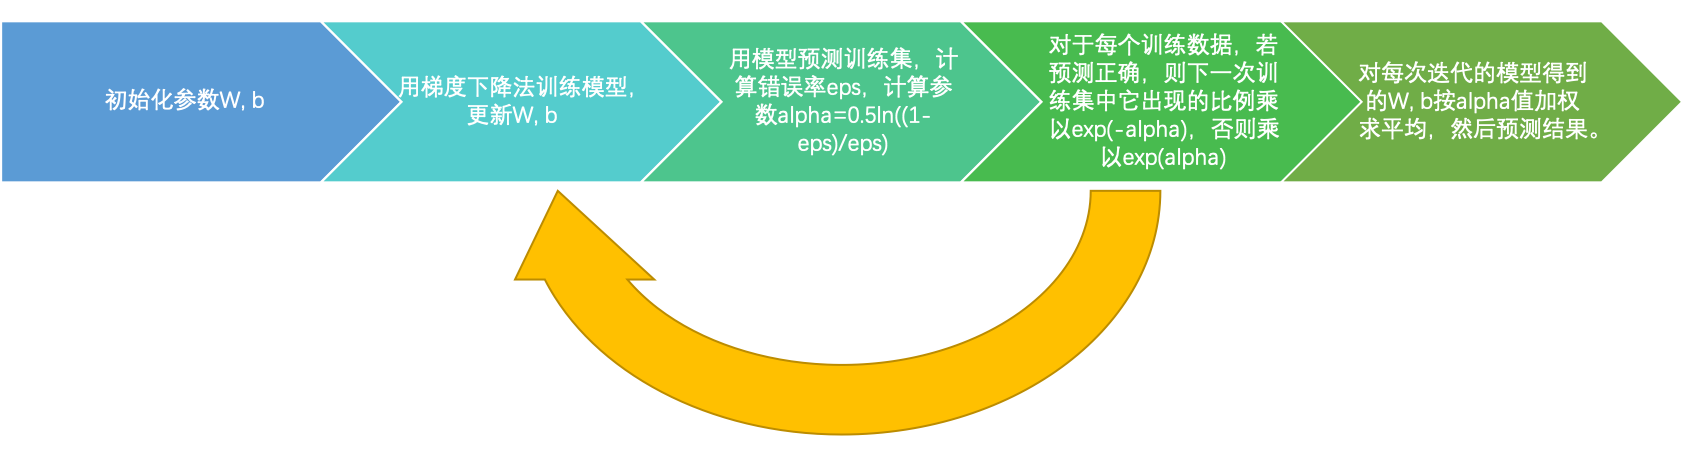
\includegraphics[scale=0.5]{5.png}
\end{figure}

线性回归模型 + AdaBoost 最好的结果为 $0.95090$ 。在测试集上,前几次迭代 AUC 还有 $0.95$ ,后面越迭代越低。它并没有超过原有的线性回归模型,至少连与它持平都做不到。

\section{总结}

我现在非常地绝望,别人交一次就能拿到 $0.98$ 以上的 AUC,而我做了那么久,却只有 $0.95$ 左右的 AUC 。

问题肯定是出在我选择的模型上。临近 Deadline ,我已无力更改模型。我只知道我尝试的两个模型(神经网络、线性回归)效果不太好, Bagging 和 AdaBoost 作用在线性回归上面的效果也不太好。我认为这很大原因是由于有些属性是离散值,用线性回归会很难使离散值发挥作用。我对离散值的处理也非常简单粗暴,先转换成整数,再转成 $[0, 1]$ 之间的实数。既然离散值是线性回归的瓶颈,那么无论用 Bagging 和 AdaBoost 再怎么跑,线性回归的准确率也不会超过这个瓶颈。决策树是能处理好离散值的一个模型,但它对连续值的处理效果也不太好。如何平衡两者,我还没试过,不知道。

通过机器学习这门课,以及第一次实验的结果,我认清了自己的方向。我不适合去科研、去玩机器学习。在这点上,我是玩不过别人的。我更适合在企业中做一些传统的算法,宁愿对着运行时间、内存调代码,也不要对着准确率换模型、调参数。

\end{document}
